\begin{figure}[htp]
	\begin{flushleft}
		The first model of the system to be presented is the model ``The world and the machine'' by M. Jackson and P. Zave. This model highlights the division between phenomena that happen entirely either in the world or in the machine, and those that are shared between the two of them.
	\end{flushleft}
	\centering
	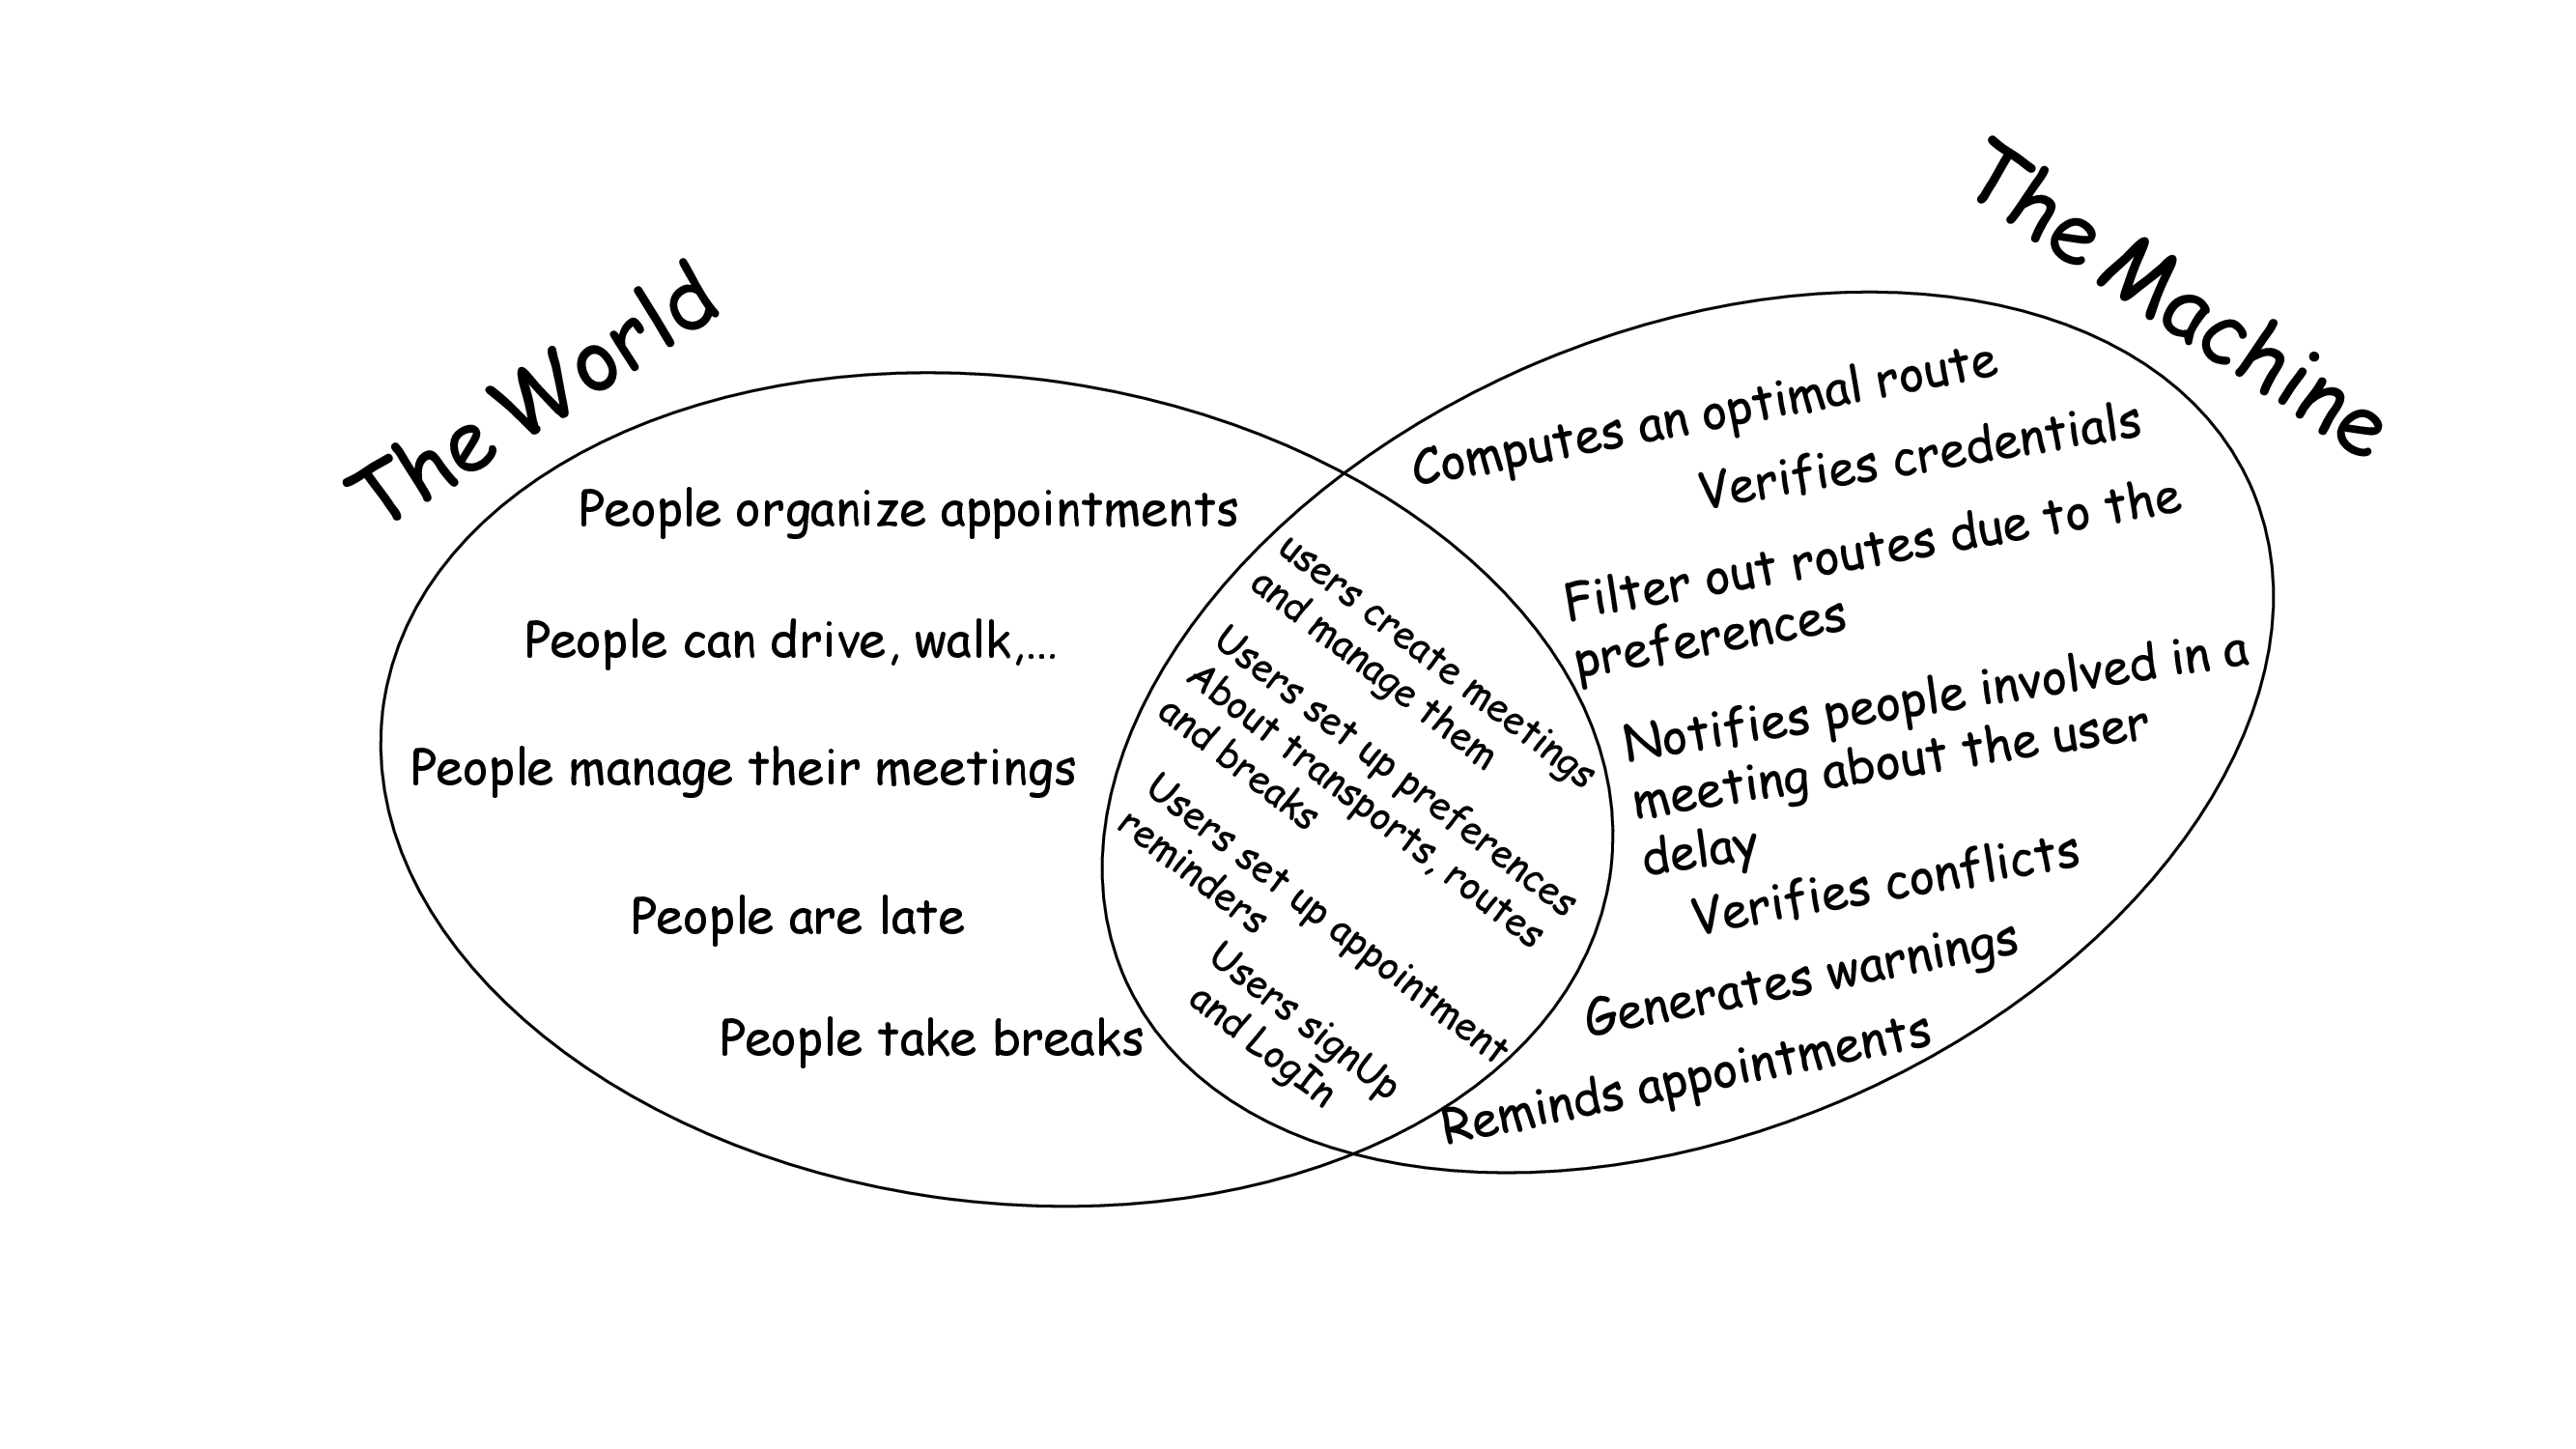
\includegraphics[width=\textwidth]{images/World-Machine}
	\caption{The world-machine chart.}
	\label{fig:world-machine}
\end{figure}
